\documentclass[11pt]{article}
\usepackage{amsmath}
\usepackage[margin=0.68in]{geometry}
\usepackage{booktabs}
\usepackage{enumitem}
\usepackage{fancyhdr}
\usepackage{graphicx}
\usepackage[table]{xcolor}
\usepackage[hidelinks]{hyperref}
\usepackage{listings}
\usepackage{microtype}
\usepackage{tabularx}
\usepackage{titlesec}
\graphicspath{{docs/lessons/assets/}{../assets/}}
\definecolor{Ink}{gray}{0}
\definecolor{CodeGray}{gray}{0.96}
\hypersetup
{
  pdftitle={ADK Lesson 025: Infrared Frame Adventure},
  pdfauthor={Kevin Shanahan},
  pdfsubject={Receive-only known NEC evidence with a visible three-frame progression},
  pdflang={en-US}
}
\pagestyle{fancy}
\fancyhf{}
\lhead{\textsc{ADK Lesson 025}}
\rhead{Infrared Frame Adventure}
\cfoot{\thepage}
\setlength{\headheight}{14pt}
\setlength{\parindent}{0pt}
\setlength{\parskip}{5pt}
\setlist{nosep,leftmargin=1.45em}
\titleformat{\section}{\Large\bfseries\color{Ink}}{}{0pt}{}
\titleformat{\subsection}{\large\bfseries\color{Ink}}{}{0pt}{}
\lstdefinestyle{adkcpp}
{
  language=C++,
  backgroundcolor=\color{CodeGray},
  basicstyle=\ttfamily\small,
  keywordstyle=\color{Ink}\bfseries,
  commentstyle=\color{Ink},
  columns=fullflexible,
  keepspaces=true,
  showstringspaces=false,
  frame=single,
  rulecolor=\color{Ink},
  breaklines=true,
  tabsize=4
}
\newcommand{\lessonbox}[1]{%
  \begin{center}\fcolorbox{Ink}{white}{\parbox{0.92\linewidth}{#1}}\end{center}}

\begin{document}
\begin{center}
  {\Huge\bfseries Infrared Frame Adventure}\\[4pt]
  {\Large Make three known button presses light a tiny victory}\\[7pt]
  \textit{Receive only. Unknown evidence never becomes a command.}
\end{center}

\begin{tabularx}{\linewidth}{@{}>{\bfseries}l X >{\bfseries}l X@{}}
Lesson & 025 --- component & Board & Arduino Mega 2560\\
Primary evidence & D45 lamp & Automatic ending & 120 seconds\\
Conditional specimen & identified receiver plus owned, harmless NEC remote\\
Status & host verified; physical observation remains open\\
\end{tabularx}

\section{The adventure}

Build one receiver and one lamp. D13 announces that every pin was acquired.
Then point an owned kit remote at the receiver. The first valid frame earns one
long glow, the second earns two flashes, and the third unlocks three quick
flashes. Unknown or damaged evidence makes a different pattern and cannot
advance the count. At two minutes the sketch turns both lamps off, releases
the pins, and waits for Reset.

\[
\text{light}\rightarrow\text{pulses}\rightarrow\text{frame}
\rightarrow\text{validity}\rightarrow\text{visible reward}
\]

\lessonbox{\textbf{Numbers are evidence, not instructions.} An address or
command field never means ``unlock'', ``open'', or ``launch''. This lesson
does not transmit, export raw captures, replay an unknown protocol, or actuate
anything beyond a resistor-limited lamp.}

\section{Specimen gate}

Use the receiver only when its own marking and a primary datasheet establish
its supply range, physical pin order, idle polarity, carrier band, and output
level. Use only an ordinary remote you own whose harmless NEC buttons are known
in advance. A similar-looking three-pin module is not an electrical identity.
If either specimen is uncertain, leave the receiver unpowered and enjoy the
deterministic software fixtures instead.

\begin{tabularx}{\linewidth}{@{}l X@{}}
\toprule
Part & Required identity\\\midrule
Mega 2560 & USB-powered board\\
Receiver & exact active-low demodulating specimen, primary datasheet reviewed\\
Remote & owned ordinary remote, known harmless NEC buttons only\\
Visible path & ordinary LED and 1 k\(\Omega\) series resistor\\
\bottomrule
\end{tabularx}

\section{Wire the literal layout}

Unplug USB before placing or moving anything. Match the Mega orientation,
header labels, breadboard letters, and numbered rows in Plate 1.

\begin{tabularx}{\linewidth}{@{}l l X@{}}
\toprule
Signal & Mega & Exact connection\\\midrule
TP-IR & D2 & identified receiver's marked OUT function\\
Receiver power & 5 V, GND & only when the exact datasheet permits 5 V\\
TP-LED & D45 & row 13a; 1 k\(\Omega\) from 13c to 13f; LED anode
  at 13h and cathode at 15h; 15j to ground rail\\
Ground rail & GND & rail to one Mega GND pin\\
\bottomrule
\end{tabularx}

\begin{center}
% ADK visual: pencil
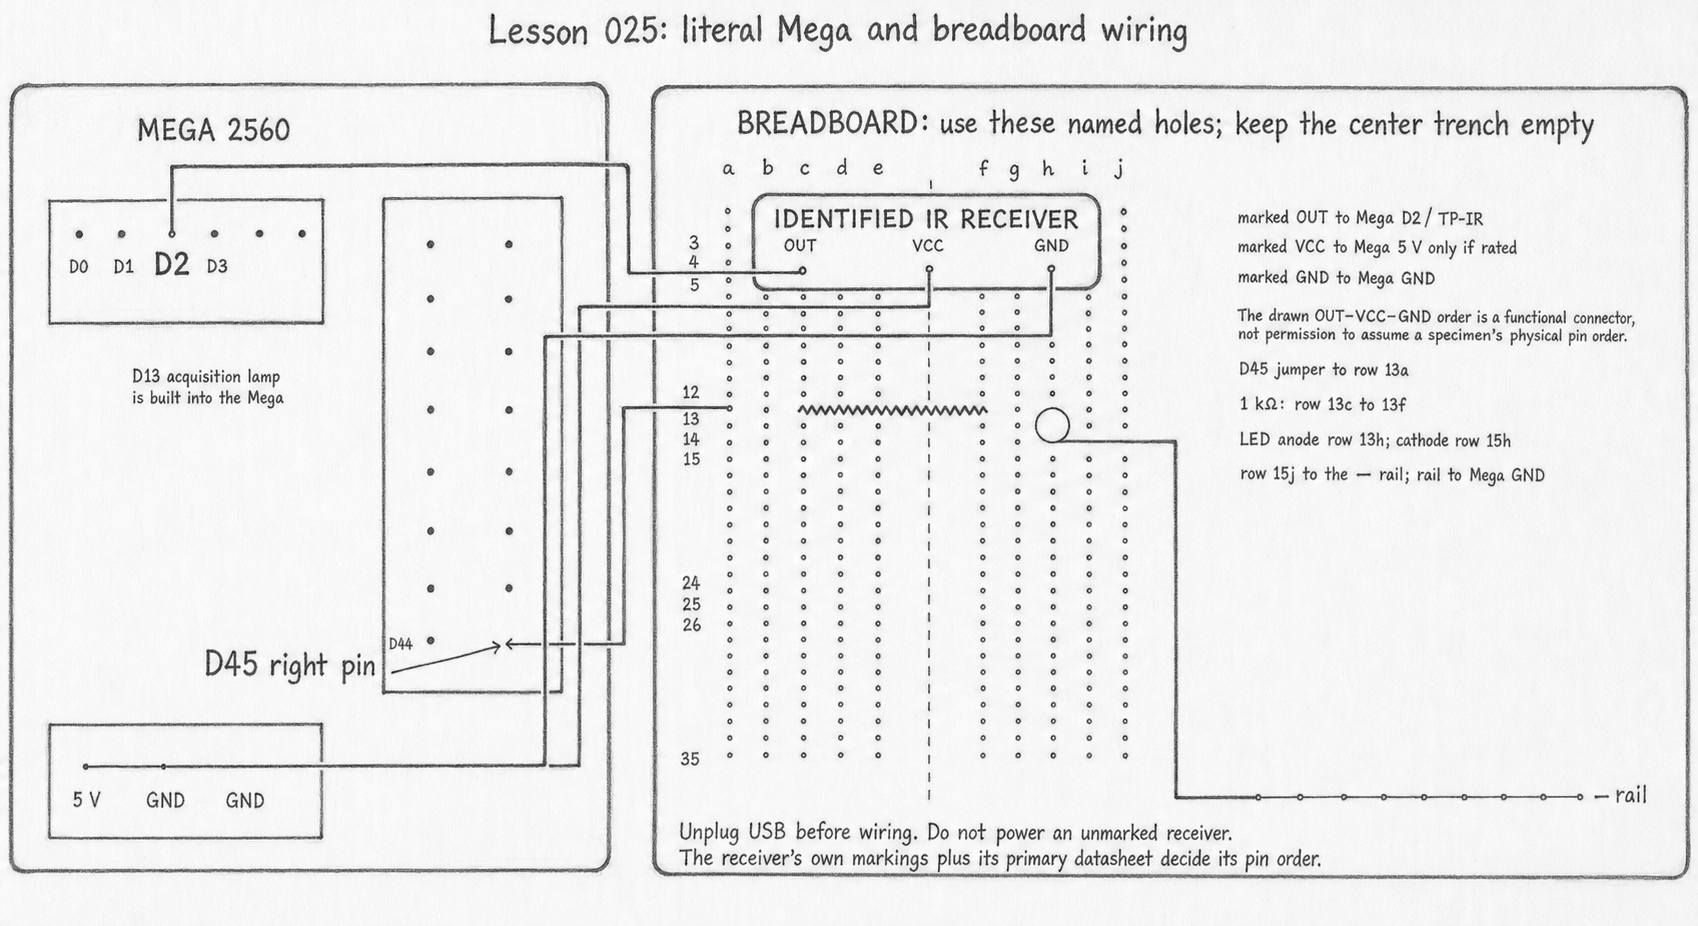
\includegraphics[width=\linewidth]{025-infrared-literal-pencil.png}

\small\textit{Plate 1 alternative text: literal Mega and breadboard plate.
D2 connects to the identified receiver OUT function. D45 reaches breadboard
row 13 through a 1 kOhm resistor and an LED spanning rows 13 and 15; the LED
cathode returns through the ground rail. Receiver VCC and GND are connected
only after its exact pin order is identified.}
\end{center}

The receiver block in Plate 1 names \emph{functions}; it deliberately does not
claim that every specimen has the drawn OUT--VCC--GND physical order. Follow
the exact specimen's marking and datasheet when mapping those three jumpers.
The breadboard LED placement, Mega headers, and occupied holes are literal.

At an illustrative 5 V rail and 2 V LED drop, the 1 k\(\Omega\) resistor limits
current to about 3 mA. Unexpected heat, unstable power, a wrong resistor, or a
voltage outside the rails means unplug immediately.

\section{Watch the story unfold}

\begin{center}
% ADK visual: pencil
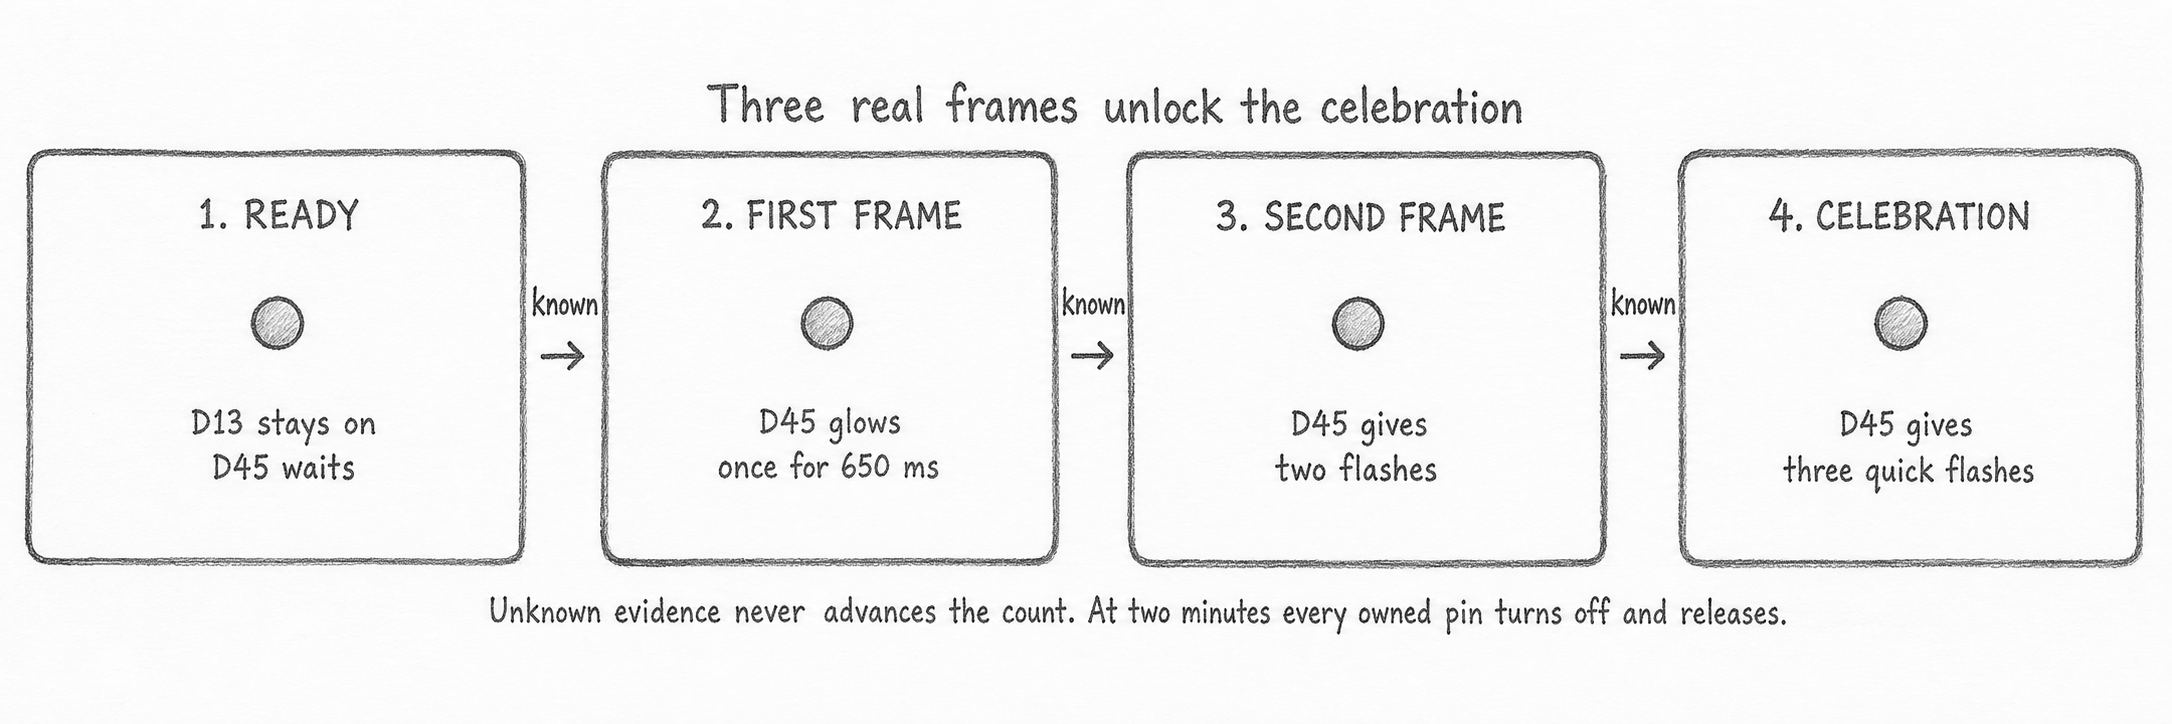
\includegraphics[width=\linewidth]{025-infrared-progress-pencil.png}

\small\textit{Plate 2 alternative text: four panels show D13 ready, one D45
glow after the first valid frame, two flashes after the second, and three
quick flashes after the third. Unknown evidence cannot advance the story.}
\end{center}

\subsection{Stage 1: ready}

After Reset, D13 stays on only if capture owns D2 and its interrupt and both
lamp endpoints initialized. D45 stays dark. That visible ready state depends
on successful resource acquisition; it does not claim receiver compatibility.

\subsection{Stage 2: find the first frame}

Press one known harmless NEC button. A valid frame makes D45 glow for 650 ms.
No Serial window is needed. If D13 is on but D45 stays dark, unplug and compare
D2, the receiver's exact pin order, LED polarity, resistor holes, and ground
return with Plate 1.

\subsection{Stage 3: unlock the progression}

Press known buttons twice more, allowing each flash story to finish. The second
valid frame produces two 250 ms flashes. The third and later valid frames
produce three 150 ms flashes. Each later reward depends on the receiver,
capture, decoder, validity decision, and earlier count all working together.

An unknown leader gives two short flashes but does not increase the valid
count. A normal NEC repeat gives one short acknowledgement and also leaves the
count unchanged. Timing, inverse-byte, overflow, or record trouble gives four
very quick flashes. Do not seek unknown transmitters to make those patterns;
automated fixtures exercise them behind the scenes.

\subsection{Stage 4: discover the fixed ending}

At 120 seconds, regardless of button activity, the sketch turns D45 and D13
off, shuts down both endpoints and capture, and waits. Reset starts a fresh
adventure. Darkness is the circuit-native ending; it is not a claim of
separately measured high impedance.

\section{How the evidence stays honest}

\texttt{PulseCapture} owns D2 and its interrupt. Its interrupt path stores only
bounded edge timestamps. A completed \texttt{PulseFrame} remains immutable
until matching acknowledgement. \texttt{InfraredDecoder} recognizes the
classic 8-bit-address NEC form, validates its leader, 32 bits, final mark, and
inverse bytes, and reports uncertainty without guessing.

\begin{tabularx}{\linewidth}{@{}l X@{}}
\toprule
Result & D45 story\\\midrule
first valid frame & one 650 ms glow\\
second valid frame & two 250 ms flashes\\
third or later valid frame & three 150 ms flashes\\
NEC repeat & one 150 ms acknowledgement; count unchanged\\
unknown protocol & two 150 ms flashes; count unchanged\\
timing, integrity, overflow, or record fault & four 100 ms flashes\\
\bottomrule
\end{tabularx}

\texttt{InfraredRecordEncoder} can also write one bounded canonical line:
\begin{verbatim}
IR1,<sequence>,<protocol>,<validity>,<address-hex>,<command-hex>\n
\end{verbatim}
Serial carries that optional record, never the primary result and never raw
replay material.

\begin{lstlisting}[style=adkcpp]
if (now.elapsedSince (adventureStarted).milliseconds () >= 120000)
{
    stopSafely ();
    return;
}

observeInfrared (adk::MicrosecondTimePoint (micros ()));
showFrameEvidence (now);
\end{lstlisting}

The automated repository suite stays behind the scenes. It covers acquisition
rollback, exact timing boundaries, repeat frames, corrupt inverse bytes,
overflow, stale acknowledgement, record capacity, timestamp wrap, shutdown,
claim reuse, and byte-identical replay. Those checks protect the adventure
without turning it into learner paperwork.

\section{Predict, observe, interpret}

Before Reset, predict that successful acquisition lights D13 while D45 remains
dark. Observe D13 after setup and interpret it only as resource-acquisition
evidence. Before each known press, predict the next D45 reward; observe at
TP-IR and D45, then interpret agreement as evidence that the receive and decode
path reached the lamp, not as general receiver compatibility. Before the
two-minute deadline, predict both lamps will go dark; observe the fixed ending
and interpret darkness only as the visible software ending. Pin release and
high impedance remain separate, unperformed physical measurements.

\section{If the visible story breaks}

\begin{tabularx}{\linewidth}{@{}l X@{}}
\toprule
What you see & Inspect while unpowered\\\midrule
D13 never lights & board power, resource conflict, then initialization path\\
D13 on; D45 always dark & receiver identity and D2, LED orientation, rows 13/15,
  resistor, ground rail\\
every press looks unknown & exact remote protocol, receiver idle polarity,
  pulse timing\\
one short flash while holding a button & normal NEC repeat; count unchanged\\
four quick flashes & timing/integrity evidence or bounded-record failure\\
progress never reaches three & use only the known buttons; allow each frame
  and visible pattern to finish\\
lamps remain on after two minutes & unplug; fixed shutdown did not complete\\
\bottomrule
\end{tabularx}

\section{Make it yours}

Put paper stars numbered 1, 2, and 3 beside D45. Change only harmless
presentation timing, or choose three named buttons on the owned remote and
write their names on the stars. Keep all numeric fields as evidence, keep
unknown evidence unable to advance, and keep the fixed two-minute ending.

\vfill\small
\textbf{Companion material.} The HTML page carries searchable pin and state
tables plus source links. This printable lesson carries the literal wiring
plate, staged visible progression, and receive-only specimen boundary.
\end{document}
